The related works highlight that presence of users, as shown by Pulijala et al. can effectively decrease trainees anxiety and stress before real operations \cite{Pulijala.2017}.
To increase the presence of users inside of VR (Requirement \ref{req::F1}), a virtual operating room has been designed with photogrammetry.

\begin{figure}[ht]
    \centering
    \begin{minipage}{.5\textwidth}
      \centering
      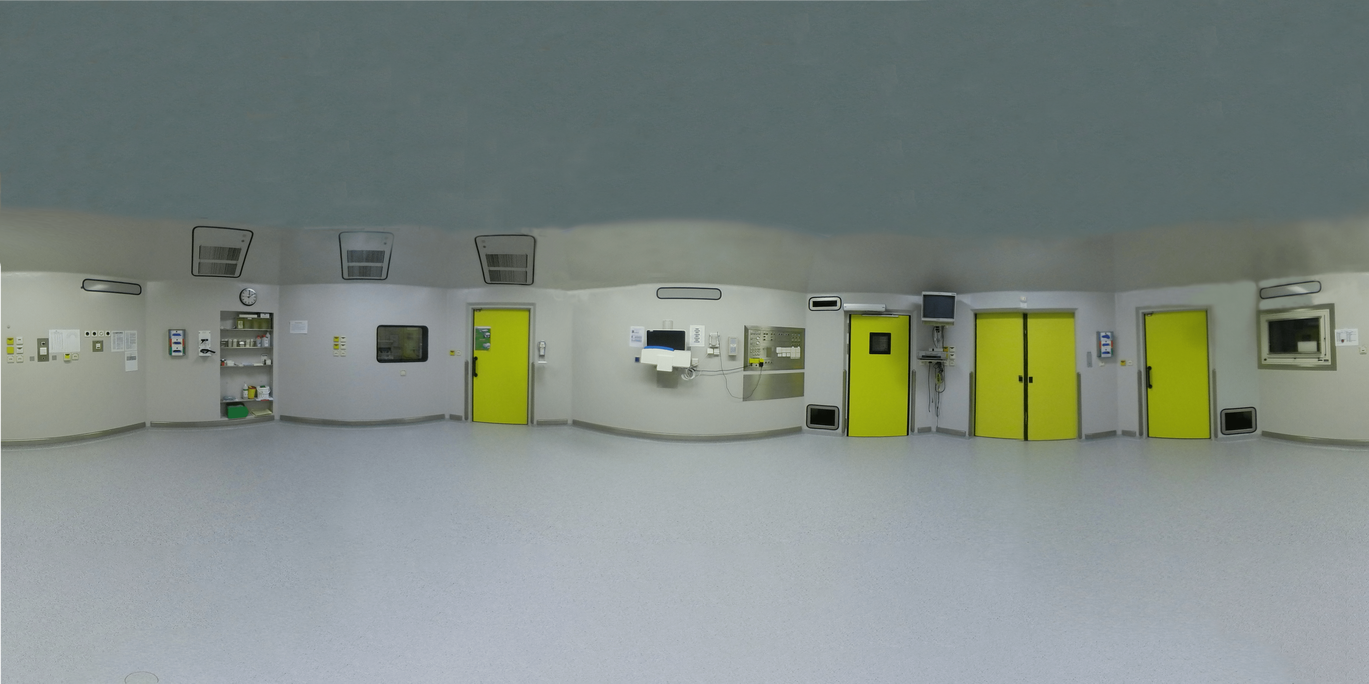
\includegraphics[width=0.99\linewidth]{images/implementation/vot/operating_room_360.png}
    \end{minipage}%
    \begin{minipage}{.5\textwidth}
      \centering
      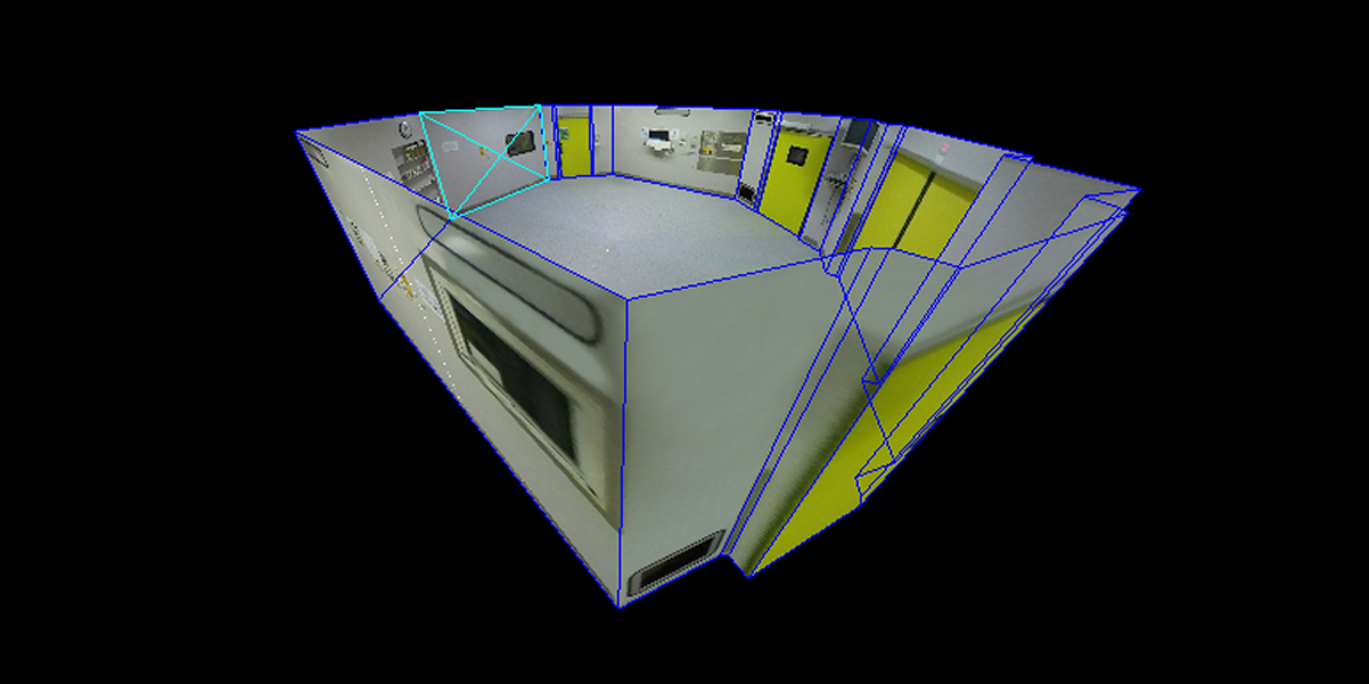
\includegraphics[width=0.99\linewidth]{images/implementation/vot/walkabout_worlds.png}
    \end{minipage}
    \caption{\label{fig::360OperatingRoom}Left: Edited 360 Degree Photograph of an OT in UHA. Right: Result of conversion to 3D model via Walkabout Worlds}
\end{figure}

The virtual operating room has been modeled with a cost-effective, simplistic
\\photogrammatry-esque approach, in which a real operation room from UHA has been captured using a 
360-degree camera (Figure \ref{fig::360OperatingRoom}), the Samsung Gear 360, and converted into a 3D model via Walkabout Worlds \cite{WalkaboutWorlds}.
For reference, the operating room 10 from UHA Aachen has been caputured and modeled for use in VR.
Beforehand, the operating room was emptied out as much as possible and then, after converting it to a 3D model, filled with freely avaliable 3D objects from open assets in Unity3D.
This way, users can feel present inside of a real OT while being able to interact with any subsequently imported 3D models found in the surgical environment.
Some details, such as the operating table dock in the middle of the room have been edited out with photo-editing software.
Note that any operating room can be modeled and added to the existing application (Requirement \ref{req::N8}).


\begin{figure}[ht]
  \centering
  \begin{minipage}{.5\textwidth}
    \centering
    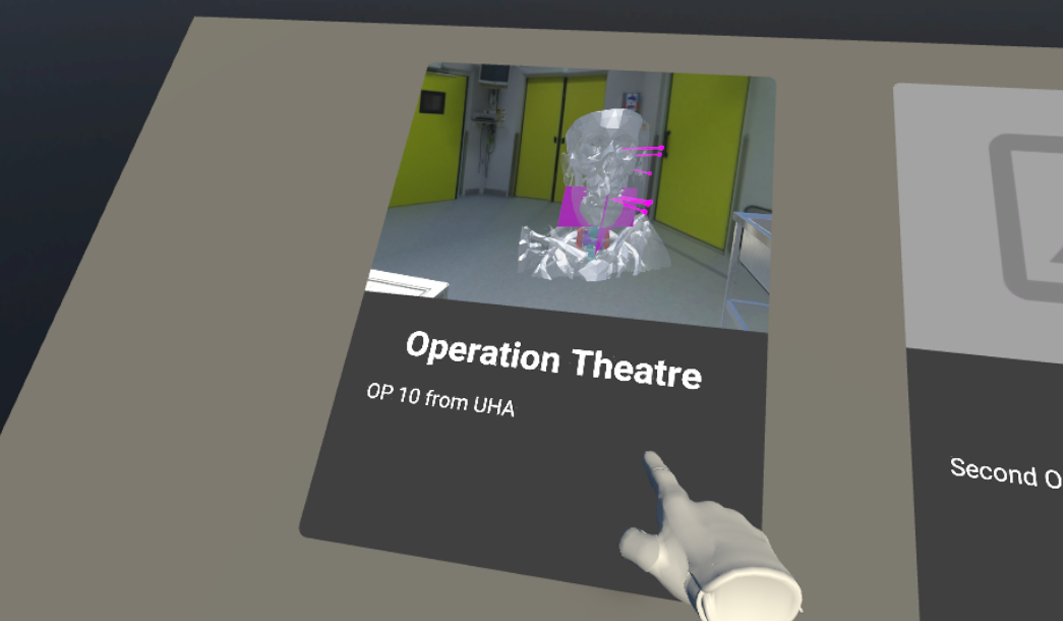
\includegraphics[width=0.99\linewidth, height=5.1cm]{images/implementation/vot/select_op.png}
  \end{minipage}%
  \begin{minipage}{.5\textwidth}
    \centering
    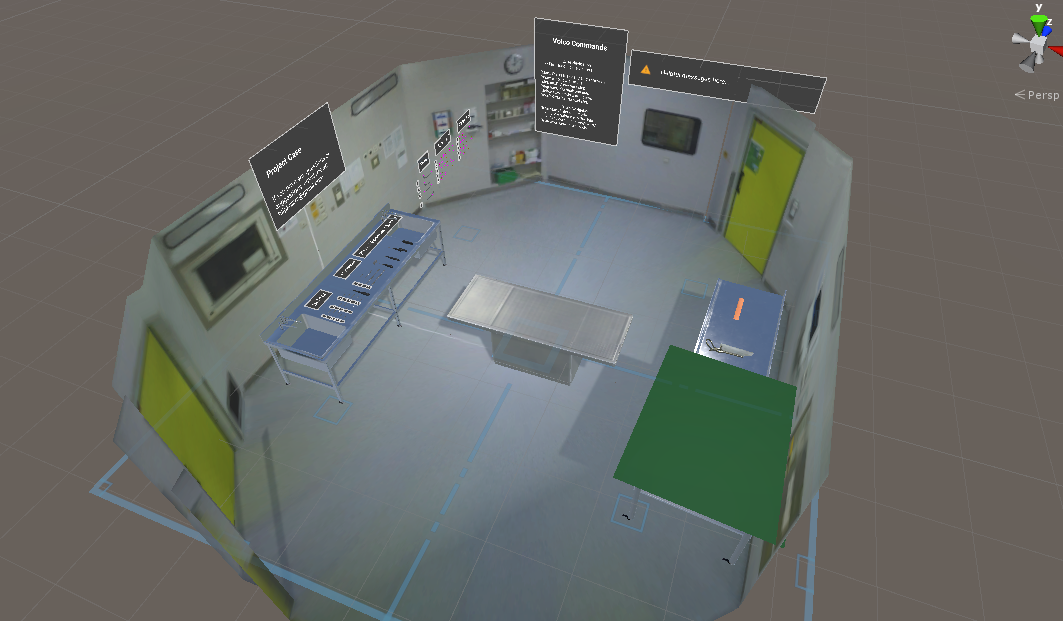
\includegraphics[width=0.99\linewidth, height=5.1cm]{images/implementation/vot/overview.png}
  \end{minipage}
  \caption{\label{fig::SceneSelect} Left: Users choose which OT they want to work in by selecting the thumbnail of an OT with their virtual hands. Right: The final virtual OT for OMFS. 
  The OT table with the patient is located in the middle. Next to it, a tray with surgical instruments.
  Textual information relevant to the procedure is floating next to the operating table.}
\end{figure}

Users can choose which OT they want to work in by selecting it in the OT select view (Figure \ref{fig::SceneSelect}).
The OT, which was created for this thesis consists of an instrument tray, where all instruments are located including their descriptive labels, the operating table, and two smaller trays 
for placing used instruments.
Additionally, information relevant to the project case is displayed inside of the OT as depicted in Figure \ref{fig::SceneSelect}.
\\ Surgical instruments were scanned via medical imaging acquisition and postprocessed in Blender3D to reduce artifacts, which occur during the 3D scanning phase of the surgical instruments and materials.
After these critical steps for immersion and presence (especially for the OMF surgeons of UHA) have been completed, instruments and materials are ready to be imported into Unity3D.
Users navigate through the OT via the locomotion options (Figure \ref{sec::Architecture}), and interact with the environment via a combination of natural gestures, GUI and VUI, as will be discussed 
extensively in the following Section.
\\ In principle, users can create their own OT and surgical instruments specialized to their medical field, import them into Unity3D, and the underlying architecture (Figure \ref{sec::Architecture}) 
will continue to work.